% !TEX encoding = UTF-8
% !TEX TS-program = pdflatex
% !TEX root = ../tesi.tex

%**************************************************************
\chapter{Progettazione e codifica}
\label{cap:progettazione-codifica}
%**************************************************************

\intro{Il seguente capitolo descrive gli strumenti e la progettazione con cui sono 
state implementate le integrazione con la \textit{web-app} \productName.}\\

%**************************************************************
\section{Tecnologie}
\label{sec:tecnologie-strumenti}

Di seguito viene data una panoramica delle tecnologie e strumenti utilizzati.

\subsection*{Java}
Java è un linguaggio di programmazione e una piattaforma di elaborazione 
rilasciato per la prima volta da Sun Microsystems nel 1995. Si è evoluto da umili
 origini per sostenere gran parte del mondo digitale di oggi, fornendo una
 piattaforma affidabile su cui sono costruiti molti servizi e applicazioni. 
 Anche i nuovi prodotti, innovativi nei servizi digitali progettati per il futuro,  
 continuano a fare affidamento su Java.
%TODO: aggiungere bibliografia, link: https://java.com/en/download/help/whatis_java.html
\subsection*{Spring}
Spring è un \textit{framework} open source per lo sviluppo di applicazioni su piattaforma Java.
A questo \textit{framework} sono associati tanti altri progetti, che hanno nomi composti come 
Spring Boot, Spring Data, Spring Batch, etc. Questi progetti sono stati ideati per
fornire funzionalità aggiuntive al \textit{framework}.
%TODO: aggiungere bibliografia, link: https://it.wikipedia.org/wiki/Spring_Framework

\subsection*{Typescript}
%**************************************************************
TypeScript è un linguaggio di programmazione sviluppato e gestito da Microsoft. 
È un \gls{superset} di JavaScript, che permette di aggiungere la tipizzazione 
statica opzionale al linguaggio. TypeScript è progettato per lo sviluppo di applicazioni 
di grandi dimensioni e per la \gls{transcompilazione} in JavaScript. Poiché TypeScript è un \gls{superset} di JavaScript, anche i programmi JavaScript esistenti sono validi programmi TypeScript.
%TODO: aggiungere bibliografia, link: https://en.wikipedia.org/wiki/TypeScript

\subsection*{Angular}
%**************************************************************
Angular è un \textit{framework} JavaScript per applicazioni \textit{web} dinamiche, utilizzato in particolare per la creazione di \gls{spa} e \textit{web-app}. Consente di utilizzare HTML come linguaggio template e di estenderne la sintassi per esprimere le componenti di un'applicazione in modo chiaro e succinto.
%TODO: aggiungere bibliografia, link: https://psicografici.com/angular-js/#:~:text=Angular%20%C3%A8%20un%20framework%20JavaScript,in%20modo%20chiaro%20e%20succinto.

\subsection*{Angular Material}
%**************************************************************
Angular Material è una libreria sviluppata da Google nel 2014 progettata per aiutare a sviluppare pagine \textit{web} in modo strutturato. \\
I suoi componenti aiutano a creare pagine \textit{web} e applicazioni \textit{web} attraenti, coerenti e funzionali.
%TODO: aggiungere bibliografia, link: https://psicografici.com/angular-js/#:~:text=Angular%20%C3%A8%20un%20framework%20JavaScript,in%20modo%20chiaro%20e%20succinto.

\subsection*{Node.js}
Node.js è una piattaforma di sviluppo open source per l'esecuzione di codice JavaScript lato \textit{server}. Node è utile per sviluppare applicazioni che richiedono una connessione permanente dal \textit{browser} al \textit{server} ed è spesso utilizzato per applicazioni in tempo reale come chat, feed di notizie e di notifiche.\\
Node.js è utilizzato da Angular per gestire le dipendenze, permettendo la dichiarazione di due insiemi di dipendenze: per gli sviluppatori e per far funzionare l'applicativo. In questo modo è possibile differenziare quali librerie si possono tralasciare in fase di \textit{deploy} dell'applicazione perché, ad esempio, necessarie solo per effettuare i test.
%TODO: aggiungere bibliografia, link: https://whatis.techtarget.com/definition/Nodejs#:~:text=James%20Denman-,Node.,feeds%20and%20web%20push%20notifications.

%**************************************************************
\section{Progettazione}
\label{sec:progettazione}

\subsection{Back end}
\subsubsection{Architettura Spring Boot}
Spring Boot è un modulo di Spring \textit{framework}. Viene utilizzato per creare applicazioni \textit{stand-alone} di livello produttivo con il minimo sforzo.\\
Spring Boot segue un'architettura a strati, in cui ogni livello comunica con gli strati vicini.\\
Ci sono quattro strati in Spring Boot sono i seguenti:
\begin{itemize}
    \item \textbf{\textit{Presentation layer}:} gestisce le richieste HTTP, trasforma il il parametro da formato JSON in classe e autentica la richiesta, per poi trasferirla al \textit{business layer};
    \item \textbf{\textit{Business Layer}:} gestisce tutta la \textit{business logic}. Consiste in classi di servizio e utilizza servizi forniti dagli strati di accesso ai dati;
    \item \textbf{\textit{Persistence Layer}:} contiene tutta la \textit{storage logic}, e trasformando gli oggetti provenienti dalla \textit{business logic} in righe del \textit{database};
    \item \textbf{\textit{Database Layer}:} in questo strato sono effettuate le operazioni \gls{CRUD}.
\end{itemize}
\begin{figure}[H] 
    \centering 
    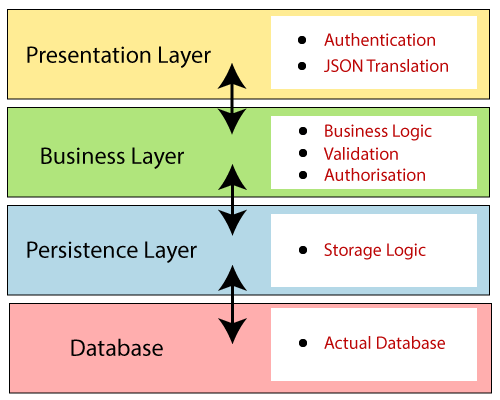
\includegraphics[scale=0.3]{spring-boot-architecture-layer.png} 
    \caption{Architettura a strati di Spring Boot}
\end{figure}

\subsubsection{Spring Boot Flow Architecture}
% https://codingjam.it/microservizi-in-java-con-spring-boot-e-spring-cloud/
\begin{figure}[H] 
    \centering 
    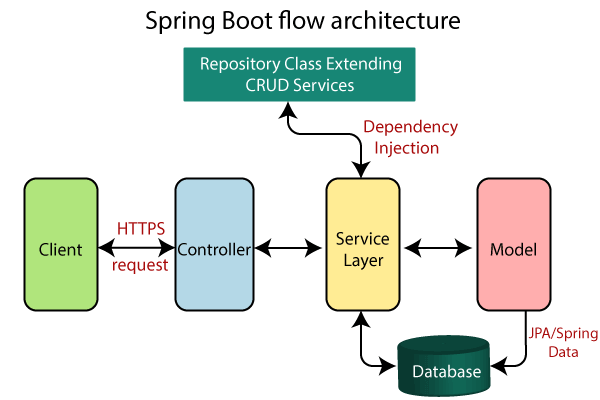
\includegraphics[width=1\columnwidth]{spring-boot-architecture.png} 
    \caption{Spring Boot \textit{workflow}}
\end{figure}
Il \textit{workflow} con cui vengono effettuate richieste HTTP utilizzando Spring Boot è il seguente:
\begin{itemize}
    \item il client esegue una richiesta HTTP (GET, POST, PUT O DELETE) ad un   \gls{endpoint} esposto;
    \item la richiesta va al \textit{controller}, che mappa la richiesta e la gestisce. Dopodiché chiama la \textit{service logic};
    \item nel \textit{service layer} viene eseguita la \textit{business logic}. Vengono eseguite le operazioni sulle classi mappate nel \textit{database};
    \item il \textit{repository} \textit{JpaRepository} esegue le operazioni sul database;
    \item una pagina \gls{JSP} viene restituita all'utente se non si è verificato un errore.
\end{itemize} 


% TODO aggiungere alla bibliografia: https://microservices.io/patterns/apigateway.html
\subsubsection{Progettazione delle API}
Il \textit{back end} del progetto è strutturato a \glspl{microservizio}, ognuno contenente una business logic atta a soddisfare un certo tipo di richieste.\\
Il \textit{front end} comunica con il \textit{back end} attraverso gli \gls{endpoint} che ogni \gls{microservizio} espone. \\
Tuttavia, effettuare connessioni dirette fra \textit{front end} e ogni \gls{microservizio} presenta alcuni problemi, come: 
\begin{itemize}
    \item numerose connessioni a seconda della quantità dei \glspl{microservizio};
    \item i \glspl{microservizio} devono esporre pubblicamente il proprio \gls{IP}, causando problemi sia di sicurezza, dovuta all'esposizione degli indirizzi IP al mondo esterno, sia in fase di latenza, ovvero il tempo che intercorre tra l'invio di una richiesta ed una risposta tenderà ad essere
    sempre più alto.
\end{itemize}

\noindent Per far fronte a queste problematiche si è deciso di utilizzare un \gls{API Gateway}.\\
In questo modo, solamente un \gls{IP} sarà visibile pubblicamente, mentre quelli dei \glspl{microservizio} possono diventare privati.\\
Per quanto riguarda la latenza il \textit{front end} comunicherà attraverso l'\gls{API Gateway}, stabilendo solo le connessioni per la richiesta e la risposta, lasciando all'\gls{API Gateway} il compito di smistare le richieste al giusto \gls{microservizio}, permettendo una connessione più rapida rispetto  all'utilizzo di connessioni diverse per ogni \gls{microservizio}, essendo tutti all'interno dello stesso \textit{network}.

\subsection{Front end}
\subsubsection{Architettura Angular}
% TODO aggiungere alla bibliografia: https://angular.io/guide/architecture
Il componente principale di Angular è il \textbf{modulo}. Un modulo è un contenitore di funzionalità che sono es
poste ad altri moduli. Questa suddivisione in moduli rende la struttura dell'applicazione ordinata e il codice mantenibile.\\
Un elemento fondamentale di Angular è il \textbf{component}, ovvero delle classi che gestiscono le \textit{view} dell'applicazione e la loro logica.\\
I dati da visualizzare nella \textit{view} vengono forniti dalle classi dette \textbf{servizi}. Queste classi svolgono diverse funzioni, come per esempio  l'esecuzione delle richieste HTTP.\\  
Ad ogni component è associato un \textit{template}, ovvero del codice HTML in cui si definisce come viene visualizzato il component.\\
È possibile personalizzare il codice HTML utilizzando le \textbf{direttive}, ovvero delle classi che aggiungono un comportamento aggiuntivo agli elementi nelle applicazioni Angular. Le direttive integrate di Angular permettono di gestire moduli, elenchi, stili e ciò che gli utenti vedono.\\
È possibile creare un component che rappresenta la pagina completa, in cui inserire diversi component per ogni elemento contenuto in quella pagina.
Ogni component contenuto si occuperà così di gestire la grafica di quella determinata funzionalità e di comunicare con i servizi di cui necessita; sarà poi il component \enquote*{padre} a gestire la disposizione dei component utilizzati. 
\subsubsection{Organizzazione del codice}
% TODO: aggiungere questa sezione alla parte di codifica
\subsubsection{Progettazione delle maschere}
Con il \textit{tutor} aziendale è stato discusso come dovrebbe essere la grafica delle nuove maschere da aggiungere a \productName. Da queste discussioni è stato poi utilizzato \nameref{sub:Figma} per fare il \textit{mockup}, in modo da  testare come i vari elementi visivi lavorano insieme.\\
Durante la progettazione del \textit{mockup} è stato seguito lo stile presente nella \textit{web-app}, in modo da non disorientare l'utente durante la navigazione. \\
I risultati della progettazione sono riportati in seguito.
\begin{figure}[H] 
    \centering 
    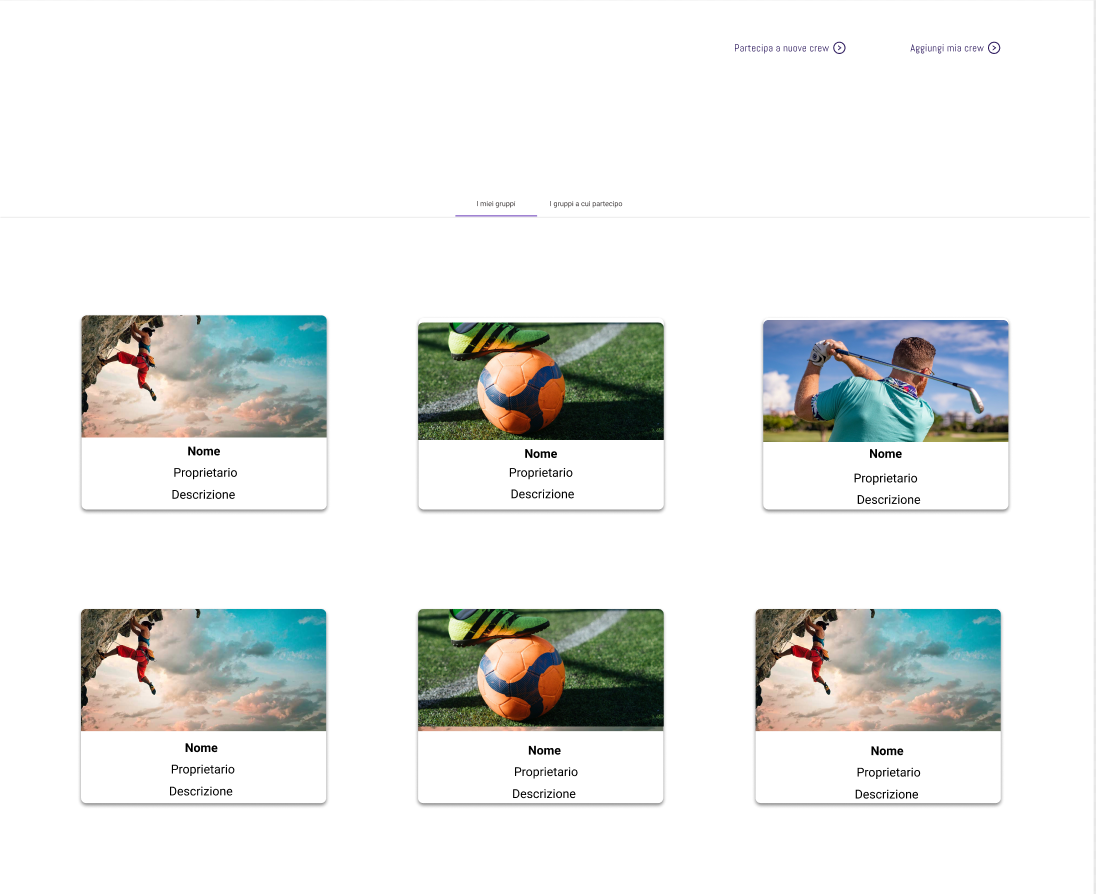
\includegraphics[scale=0.6]{mockup/le-mie-crew.png} 
    \caption{Mockup pagina per la visualizzazione dei gruppi creati dall'utente}
\end{figure}

\begin{figure}[H] 
    \centering 
    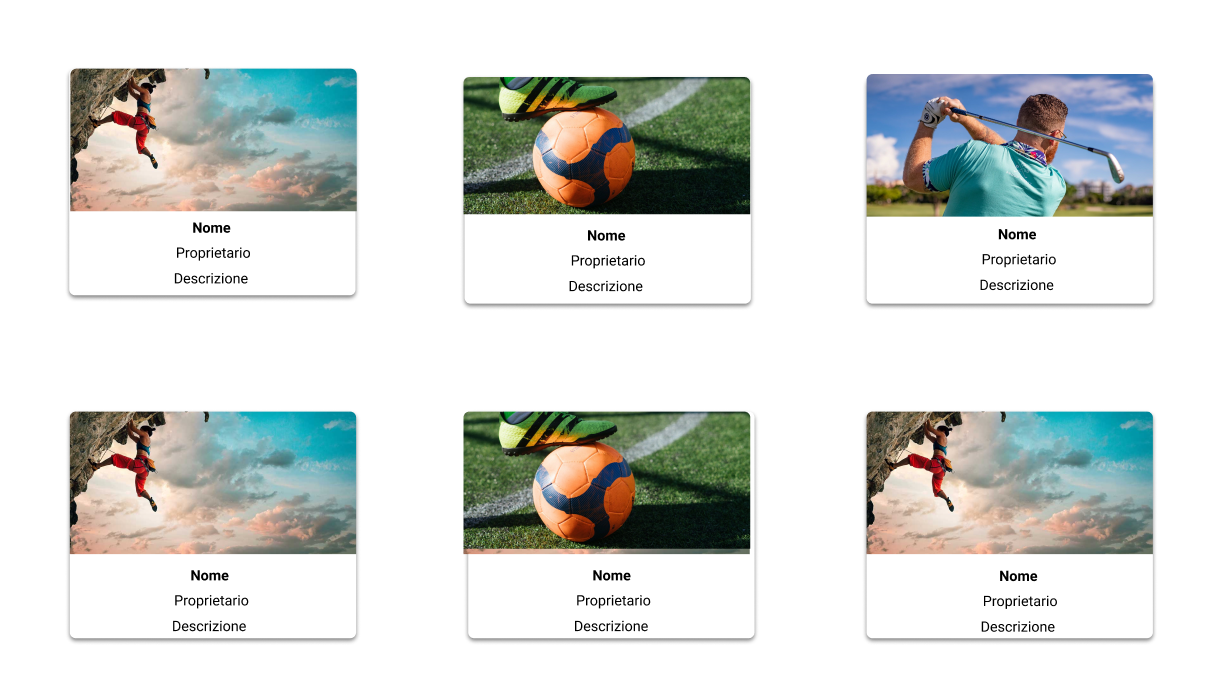
\includegraphics[scale=0.6]{mockup/lista-crew.png} 
    \caption{Mockup pagina per la visualizzazione dei gruppi a cui partecipa l'utente}
\end{figure}

\begin{figure}[H] 
    \centering 
    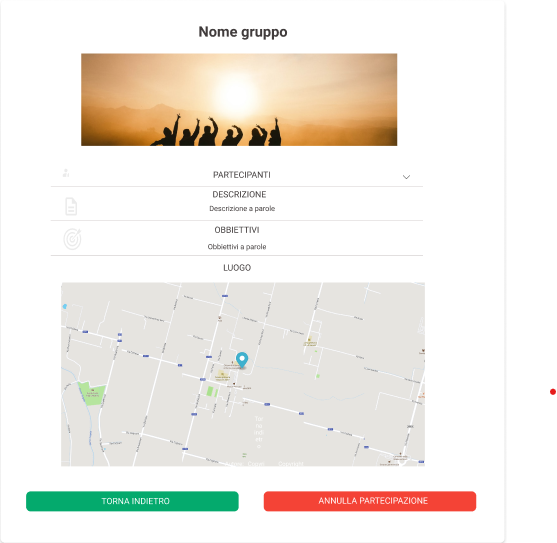
\includegraphics[scale=0.54]{mockup/dettagli-crew.png} 
    \caption{Mockup pagina per la visualizzazione dei dettagli di un gruppo}
\end{figure}

\begin{figure}[H] 
    \centering 
    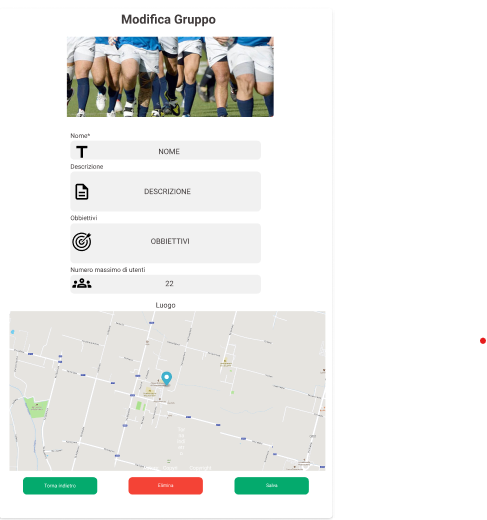
\includegraphics[scale=0.54]{mockup/modifica-crew.png} 
    \caption{Mockup pagina per la modifica dei dettagli di un gruppo}
\end{figure}

Come si può notare dalle immagini, sono stati omessi dalla progettazione l'header e il footer, in quanto sono già presenti nella \textit{web-app}.


% \subsubsection{Namespace 1} %**************************
% Descrizione namespace 1.

% \begin{namespacedesc}
%     \classdesc{Classe 1}{Descrizione classe 1}
%     \classdesc{Classe 2}{Descrizione classe 2}
% \end{namespacedesc}


%**************************************************************
\section{Design Pattern utilizzati}
\subsection{Microservizi}
% TODO: aggiungere alla bibliografia: https://aws.amazon.com/it/microservices/
I \glspl{microservizio} sono un approccio per lo sviluppo e l'organizzazione dell'architettura \textit{software} secondo cui quest'ultimi sono composti di servizi indipendenti di piccole dimensioni che comunicano tra loro tramite \gls{API} ben definite.\\
Nel contesto di questo progetto, sono stati implementati tre \glspl{microservizio}: 
\begin{itemize}
    \item \textbf{SW\_Gruppi}: \gls{microservizio} responsabile per la gestione delle funzionalità legate ai gruppi;
    \item \textbf{ApiGateway}: \gls{microservizio} che implementa il \textit{pattern} \nameref{sub:ApiGateway};
    \item \textbf{EurekaServer}: \gls{microservizio} che implementa il pattern \hyperref[sub:ServiceRegistry]{ServiceRegistry}. 
\end{itemize}
\subsection{API Gateway}
\label{sub:ApiGateway}
\begin{figure}[H] 
    \centering 
    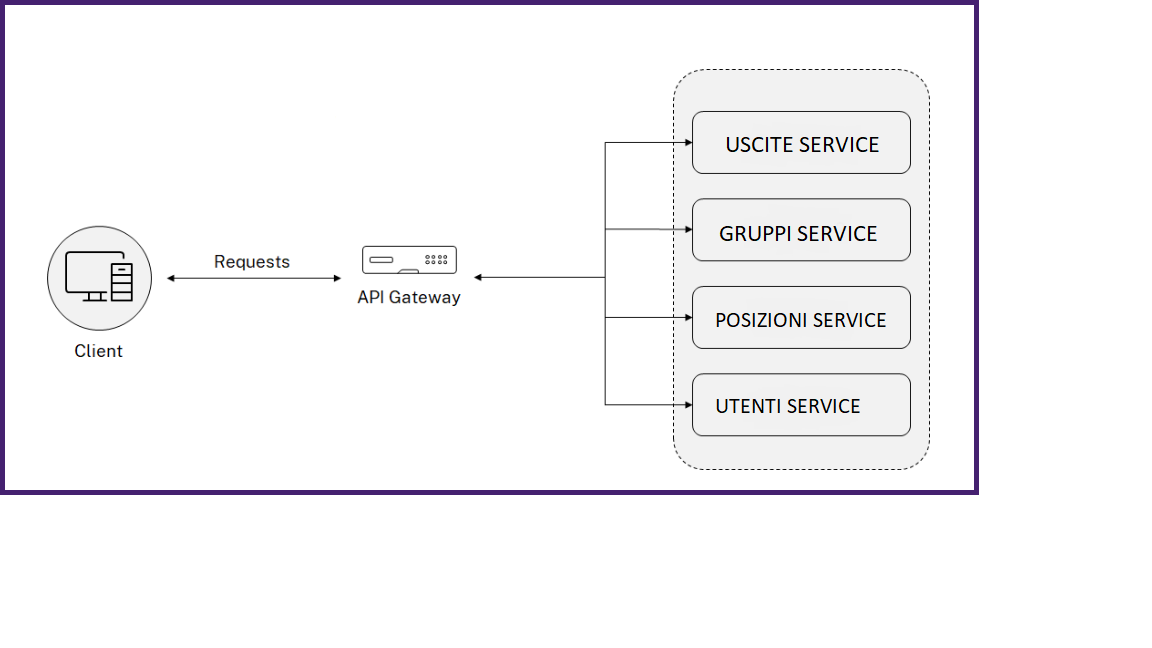
\includegraphics[scale=0.68]{progettazione/API-Gateway.png} 
    \caption{Diagramma concettuale che descrive l'API Gateway}
\end{figure}
Un \gls{API Gateway} è uno strumento di gestione delle \gls{API} che si situa tra un \textit{client} e una raccolta di servizi \textit{back end}. Un \gls{API Gateway} si comporta come un \textit{proxy} inverso per riceve tutte le chiamate \gls{API}, aggregando le chiamate alle \gls{API} dei servizi richiesti, gestendo e restituendo i risultati appropriati in base alle richieste ricevute.\\
Utilizzare un \gls{API Gateway} è vantaggioso perché: 
\begin{itemize}
    \item permette di centralizzare il punto di ingresso per le chiamate;
    \item permette di monitorare le risorse utilizzate;
    \item permette di proteggere un servizio che è aperto a tutti;
    \item ha latenza minore rispetto alla chiamata a diversi servizi.
\end{itemize}

\subsection{Client-Side Service Discovery e Service Registry}
\label{sub:ServiceRegistry}
\begin{figure}[H] 
    \centering 
    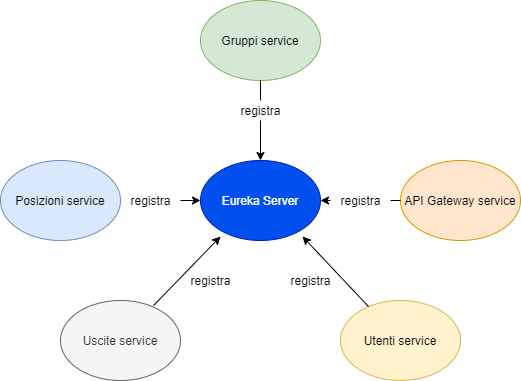
\includegraphics[scale=0.4]{progettazione/registrazione-servizi.png} 
    \caption{Diagramma concettuale che descrive la registrazione dei microservizi all'Eureka Server}
\end{figure}
%TODO: aggungere bibliografia: https://lalverma.medium.com/spring-boot-microservices-implementing-service-discovery-cfc98e49b74f, https://microservices.io/patterns/service-registry.html
I \glspl{microservizio} hanno una natura dinamica, in quanto è possibile che più istanze di un singolo \gls{microservizio} coesistano, probabilmente esponendo le loro \gls{API} in un indirizzo \gls{IP} diverso o in una porta diversa. Queste evenienze portano all'impossibilità di: 
\begin{itemize}
    \item conoscere la posizione di qualsiasi istanza dei \glspl{microservizio};
    \item tenere traccia di tutte le istanze;
    \item selezionare un'istanza di \gls{microservizio}.
\end{itemize}
La soluzione a questi problemi è l'utilizzo del \textit{pattern} \textbf{\textit{Client-side Service Discovery}}, che fornisce un meccanismo che tiene traccia di tutti i servizi e delle relative istanze. Tutti i \glspl{microservizio} si registrano ad un \textit{Service registry} e continuano ad aggiornare regolarmente le proprie informazioni di rete.\\
Il \textit{pattern} \textbf{\textit{Service registry}} è stato applicato mediante l'implementazione di un \class{Eureka Server}. L'\textit{Eureka Server} è un \textit{database} di servizi che tiene traccia di ogni \gls{microservizio}, delle loro istanze e delle loro locazioni. I \glspl{microservizio} si registrano all'avvio dell'applicazione e vengono rimossi alla sua chiusura.\\
L'utilizzo di questi \textit{pattern}  permette ai servizi di comunicare fra di loro, ottenendo le informazioni degli altri servizi direttamente dall'Eureka Server.
\subsection{MVC}
% TODO: da fare
\subsection{Dependency Injection}
\label{sub:Dependency-Injection}
% TODO: aggiungere alla bibliografia: https://davioooh.com/blog/2017/08/19/spring-dependency-injection
Sia Angular sia Spring sono dei \textit{framework} che implementano delle convenzioni che permettono l'utilizzo del \textit{patter} \class{Dependency Injection}.\\
L'ecosistema all'interno del quale le applicazioni Spring vivono viene definito \textbf{IoC container}. Lo \textit{IoC container} si occupa di istanziare gli oggetti (\textit{beans}) dichiarati nel progetto e di reperire e iniettare tutte le dipendenze ad essi associate. Tali dipendenze possono essere componenti del \textit{framework} o altri \textit{bean} dichiarati nel contesto applicativo.\\
La dichiarazione di una classe come componente nel progetto avviene tramite l'utilizzo dell'annotazione \code{@Component}, che rappresenta la categoria più generica per la dichiarazione di un componente.
Durante la fase di codifica del progetto sono state utilizzate le annotazioni \code{@Controller}, \code{@Service} e \code{@Repository}, che sono delle specializzazioni dell'annotazione \code{@Component}.\\
Per iniettare delle classi da recuperare dal \textit{IoC container} è sufficiente utilizzare l'annotazione \code{@Autowired}.
\begin{figure}[H] 
    \centering 
    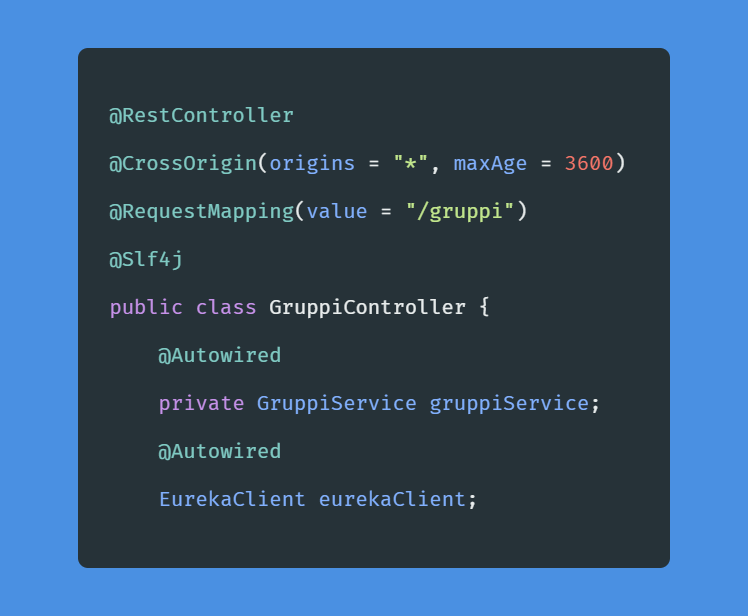
\includegraphics[scale=0.2]{progettazione/autowired-code.png}
    \caption{Esempio di Dependency Injection con Spring}
\end{figure}
% TODO: aggiungere alla bibliografia: https://angular.io/guide/dependency-injection
\noindent Angular permette l'utilizzo della \textit{Dependency Injection} di tipo \textit{constructor}, che prevede che una classe dichiari nel costruttore le dipendenze di cui ha bisogno che in fase di inizializzazione gli verranno fornite.\\
Angular include un meccanismo di \textit{Dependency Injection} davvero solido e molto flessibile, il cui utilizzo si può riassumere in due semplici passi: si crea il servizio e si inietta la dipendenza ove necessario.\\
Nel dettaglio, le fasi sono le seguenti: 
\begin{itemize}
    \item si crea un servizio, ovvero una classe Angular, che viene annotata come \code{@Injectable}. Di \textit{default}, questo decoratore ha una proprietà \code{ProvideIn}, che crea un \textit{provider} per il servizio. Nel caso, per esempio, di \code{ProvideIn: `root'}, viene specificato  che Angular dovrebbe fornire il servizio nella \textit{root injector}, ovvero diponibile a tutte le classi;
    \begin{figure}[H] 
        \centering 
        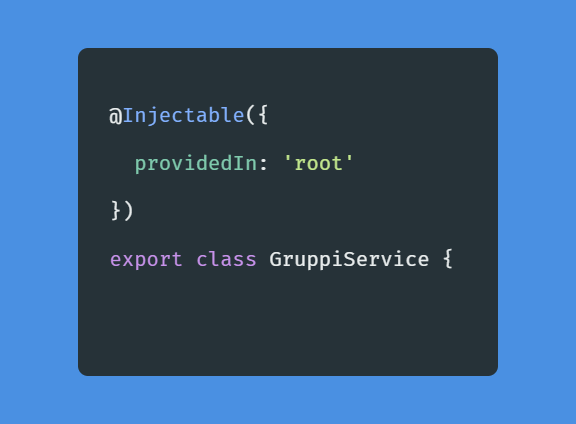
\includegraphics[scale=0.2]{progettazione/injectable.png}
        \caption{Esempio di creazione di un servizio}
    \end{figure}
    \item  si inietta il servizio e lo si utilizza ovunque sia necessario.
    \begin{figure}[H] 
        \centering 
        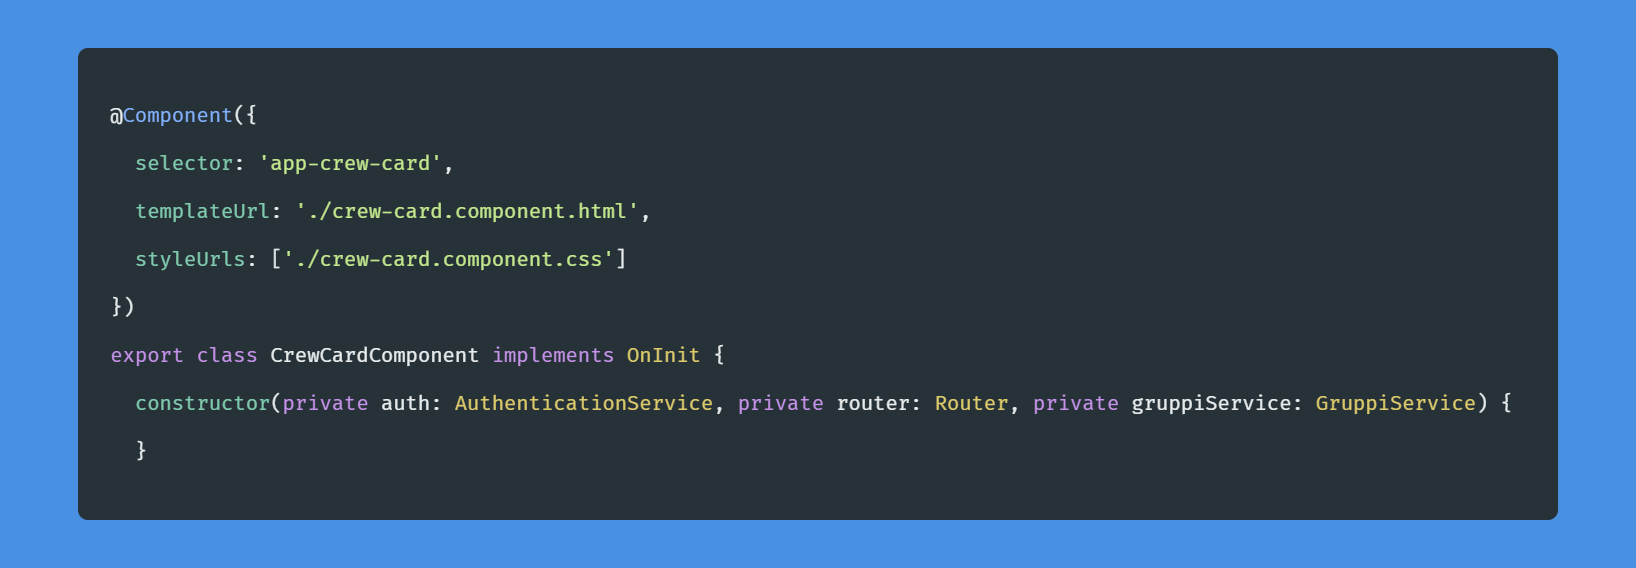
\includegraphics[scale=0.2]{progettazione/injected-service.png}
        \caption{Esempio di \textit{constructor injection}}
    \end{figure}
\end{itemize}
\subsection{Singleton}
\label{sub:Singleton}
%TODO: aggiungere alla bibliografia: https://refactoring.guru/design-patterns/singleton
Angular e Spring integrano fra i loro \textit{pattern} il \class{Singleton}, che viene implementato mediante l'utilizzo della \nameref{sub:Dependency-Injection}.\\
Utilizzando questo \textit{pattern} è stato possibile creare una sola istanza di una classe, potendola utilizzare fra i vari servizi e componenti.\\
L'utilizzo del \textit{pattern Singleton}, tuttavia, potrebbe violare il \gls{SRP}, rendendolo un \textit{anti-pattern}. Nel contesto del progetto di \textit{stage}, questo \textit{pattern} è stato utilizzato per le classi di tipo \textit{Controller}, \textit{Service} e \textit{Repository}. In questo caso il suo utilizzo è necessario in quanto sarebbe logicamente sbagliato avere più istanze per il tipo di classi sopra citate.

\subsection{Feature Service}
%TODO: aggiungere alla bibliografia: https://angular.io/guide/feature-modules
Questo \textit{pattern} è utilizzato da Angular per estrarre da una classe di tipo \textit{Component} la sua relativa logica, che può essere per esempio la visualizzazione dei dettagli di un gruppo.\\
 Mediante l'utilizzo del \textit{pattern} \nameref{sub:Singleton} e \nameref{sub:Dependency-Injection} è possibile utilizzare i vari componenti in tutti i componenti dell'applicazione.
\subsection{Lazy Loading}
%TODO: aggiungere alla bibliografia: https://angular.io/guide/lazy-loading-ngmodules
Questo \textit{pattern} è utilizzato da Angular per caricare i moduli solo nel momento in cui effettivamente vengono utilizzati, ottenendo così bassa la quantità di dati scaricata dall'utente iniziale e una diminuzione del tempo necessario al caricamento dell'applicazione.\\
Viene utilizzato questo \textit{pattern} per la gestione del \textit{routing}, associando ad una specifica \textit{view} dell'applicazione un \textit{path} di navigazione presente nella \gls{URL}.
\begin{figure}[H] 
    \centering 
    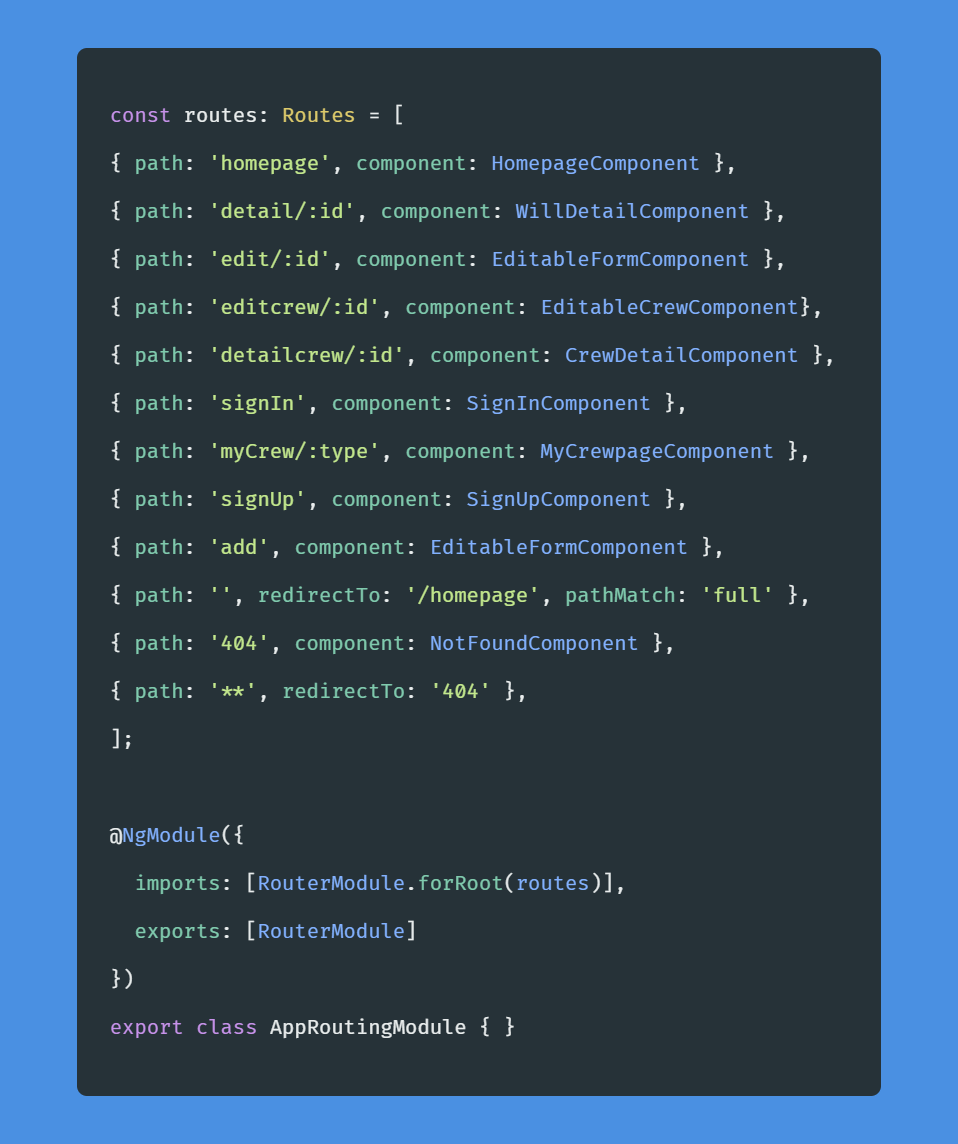
\includegraphics[scale=0.3]{progettazione/routing.png}
    \caption{Implementazione del \textit{pattern} \textit{Lazy loading} nel \class{AppRoutingModule}}
\end{figure}
\subsection{Observer}
%TODO: aggiungere alla bibliografia: https://angular.io/guide/observables
Gli \textit{\textbf{Observable}} forniscono supporto per il passaggio di messaggi tra le parti dell'applicazione. Sono usati frequentemente in Angular e sono una tecnica per la gestione ad eventi e la programmazione asincrona.\\
Il \textit{pattern Observer} è un \textit{design pattern} in cui un oggetto, chiamato \class{Subject}, contiene una lista di suoi osservatori, chiamati \class{Observers}, e li notifica automaticamente ai cambiamenti di stato.\\
Gli \textit{Observable} sono dichiarativi, ovvero viene definita una funzione che non viene eseguita fino a quando un \textit{Observer} si sottoscrive ad esso. L'\textit{Observer} viene quindi notificato al completamento della funzione, e il tipo di ritorno di un \textit{Observable} può cambiare in base al contesto, che nel caso nel progetto di \textit{stage} è stato prevalentemente di tipo HTTP \textit{response}. \\
\begin{figure}[H] 
    \centering 
    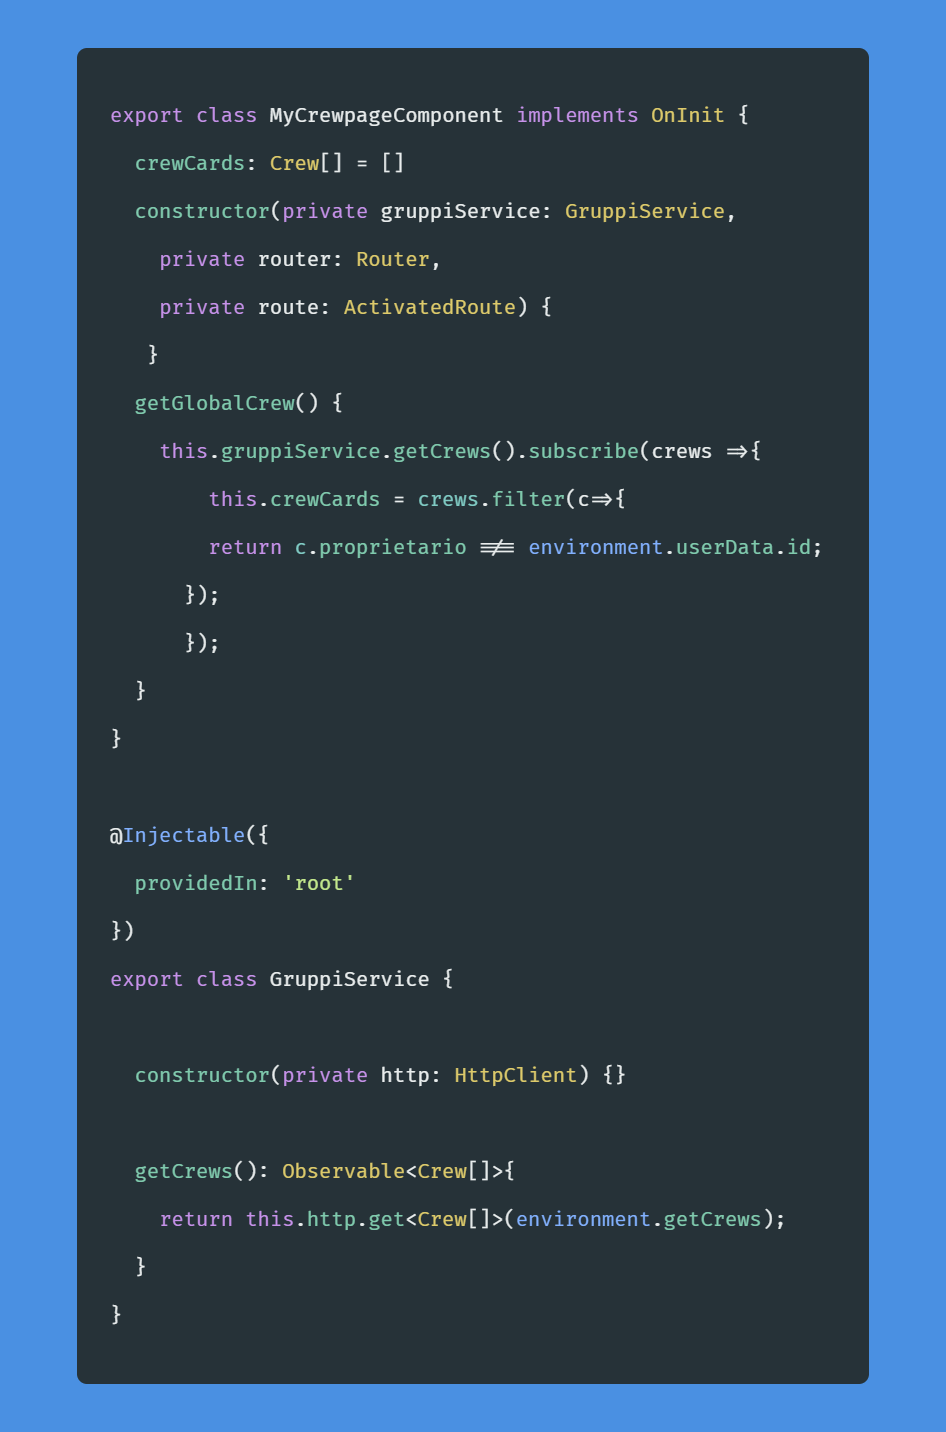
\includegraphics[scale=0.28]{progettazione/subscribe-example.png}
    \caption{Esempio implementazione \textit{pattern Observer}}
\end{figure}
\newpage
%**************************************************************
\section{Codifica}
\subsection{Back end}
\subsubsection{Gruppi service}
\myparagraph{GruppiController}
% TODO: aggiungere immagine della classe
Classe che permette di esporre le \gls{API} mappate nel \textit{path} \texttt{/gruppi}. 
L'annotazione \code{@RestController} permette di creare un \textit{controller Restful}, e l'oggetto da restituire viene serializzato automaticamente in JSON e restituito all'oggetto di risposta HTTP.
\subparagraph*{Metodi principali}
\begin{itemize}
    \item \class{getAllGruppi}: gestisce la chiamata che visualizza tutti i gruppi.\\ \mappaturaemetodo{/}{GET};
    \item \class{getGruppo}:  gestisce la chiamata che visualizza uno specifico gruppo. \\ \mappaturaemetodo{/\{id\}}{GET};
    \item \class{getUtentiByGruppo}: gestisce la chiamata che visualizza gli utenti di un appartenenti ad un gruppo. \\ \mappaturaemetodo{/\{idCrew\}/utenti}{GET};
    \item \class{createGruppo}: gestisce la chiamata che inserisce una nuovo gruppo. \\ \mappaturaemetodo{/inserisci}{POST};
    \item \class{modifyGruppo}: gestisce la chiamata che modifica un gruppo.\\ \mappaturaemetodo{/modifica/\{idCrew\}}{PUT};
    \item \class{getUsciteByGruppo}: gestisce la chiamata che visualizza le uscite di una gruppo.\\ \mappaturaemetodo{/\{idCrew\}/uscite}{GET};
    \item \class{deleteGruppo}: gestisce la chiamata che elimina un gruppo. \\ \mappaturaemetodo{/elimina/\{idCrew\}}{DELETE};
    \item \class{getGruppiUtente}: gestisce la chiamata che richiede tutti i gruppi a cui appartiene un utente. \\ \mappaturaemetodo{/utente/\{idUtente\}}{GET};
    \item \class{addUtenteToGruppo}: gestisce la chiamata che permette ad un utente di unirsi ad un gruppo. \\ \mappaturaemetodo{/\{idCrew\}/aggiungi/utente/\{idUtente\}}{POST};
    \item \class{removeUtenteFromGruppo}: gestisce la chiamata che permette ad un utente di rimuoversi da un gruppo. \\ \mappaturaemetodo{\{idCrew\}/elimina/utente/\{idUtente\}}{DELETE};
    \item \class{addUscitaToGruppo}:  gestisce l'aggiunta di un uscita ad un gruppo. \\ \mappaturaemetodo{/\{idCrew\}/aggiungi/uscita/\{idUscita\}}{POST};
    \item \class{removeUscitaFromGruppo}: gestisce l'eliminazione di un uscita ad un gruppo. \\ \mappaturaemetodo{/\{idCrew\}/elimina/uscita/\{idUscita\}}{DELETE}.  
\end{itemize}


\myparagraph{GruppiService}
% TODO: aggiungere immagine della classe
Classe responsabile della \textit{business logic} del \gls{microservizio}.  \\
Siccome fornisce funzionalità di \textit{business}, questa classe è annotata con l'annotazione \code{@Service}, ed ha lo scopo di fungere da intermediario fra la classe \class{GruppiController} e  il \gls{DAO}, ovvero le classi \hyperref[CrewRepository]{CrewRepository}, \hyperref[JointUtentiCrewRepository]{JointUtentiCrewRepository} e \hyperref[JointUsciteCrewRepository]{JointUsciteCrewRepository}. 

\myparagraph{Repository}
\label{Repository}
Interfacce con funzionalità \gls{JPA} che permettono di mappare una classe in una tabella di un \textit{database} relazionale, svolgendo anche il compito \gls{EntityManager}, effettuando l'accesso agli oggetti ed eseguendo operazioni \gls{CRUD} sui dati immagazzinati nelle tabelle del \textit{database}.\\
Tutte queste interfacce estendono l'interfaccia \code{JpaRepository<T,ID>}, dove T è il tipo della classe da mappare, ed ID è il tipo dell'identificativo della classe mappata.\\
L'interfaccia \textit{JpaRepository} permette di creare le \textit{query} a partire dal nome del metodo, senza doverlo necessariamente implementare.\\
Il meccanismo che permette di generare le \textit{query} integrato nell'infrastruttura \textit{JPA Spring Data} è utile per creare \textit{query} vincolante sulle entità del \textit{repository}. Questo meccanismo rimuove i prefissi \textit{find...By}, \textit{read...By} e \textit{get...By} dal metodo ed effettua il \textit{parsing} della funzione alla ricerca dei nomi delle proprietà dell'entità mappata nel \textit{JpaRepository}, come nel seguente esempio: 
\begin{center}
    \code{Crew findById(int id);}
\end{center}
in cui \textit{id} è una proprietà dell'entità \class{Crew}.\\ 
 Le proprietà inserite nel nome del metodo possono essere concatenate con \textit{And} e \textit{Or}, ma anche con operatori come \textit{Between}, \textit{LessThan}, \textit{GreaterThan}, \textit{Like}. \\
 Un esempio è il seguente: 
 \begin{center}
     \code{long deleteByIdUscitaAndIdCrew (int idUscita, int idCrew);}
 \end{center}
È possibile applicare l'ordinamento statico aggiungendo una clausola \textit{OrderBy} al metodo di \textit{query} facendo riferimento ad una proprietà, come nel seguente caso:  
\begin{center}
    \code{List<Crew> findByOrderById()};
\end{center}
Ci sono tre \textit{repository} nel \gls{microservizio}: \class{JointUsciteCrewRepository, JointUtentiCrewRepository} e \class{CrewRepository}. 
\mysubparagraph{JointUsciteCrewRepository} 
\label{JointUsciteCrewRepository}
\textit{Repository} che contiene le uscite di un gruppo. Ogni qualvolta un utente aggiunge un uscita, essa viene aggiunta alle uscite di tutti i gruppi a cui appartiene. Viceversa quando viene eliminata un'uscita viene eliminata dalle uscite di tutti i gruppi.\\
Un accorgimento che è stato fatto è che quando viene rimosso un gruppo, tutte le uscite associate a quel gruppo vengono rimosse da questa tabella (n.b. le uscite non vengono eliminate dalla tabella Uscite presente nel \textit{database}, vengono solo eliminate le voci relative nella tabella \textit{joint\_uscite\_crew}).
\subsubparagraph{Metodi}
\begin{itemize}
    \item \class{List<JointUsciteCrew> findAllByIdCrew(int idCrew)}: restituisce tutte le occorrenze in base all'id del gruppo;
    \item \class{Long deleteByIdUscitaAndIdCrew (int idUscita, int idCrew)}: elimina le occorrenze in base all'id del gruppo e all'id dell'uscita. Ritorna il numero di occorrenze eliminate (che sono al più una);
    \item \class{JointUsciteCrew getByIdUscitaAndIdCrew(int idUscita, int idCrew)}: restituisce un'occorrenza in base all'id dell'uscita e all'id del gruppo;
    \item \class{Long deleteByIdCrew(int idCrew)}: elimina tutte le occorrenze in base all'id del gruppo. Ritorna il numero di occorrenze eliminate;
    \item \class{void deleteByIdUscita(int idUscita)}: elimina tutte le occorrenze in base all'id dell'uscita.
\end{itemize}

%TODO: riportare un esempio con un immagine





\mysubparagraph{JointUtentiCrewRepository}
% TODO: aggiungere immagine della classe
\label{JointUtentiCrewRepository}
\textit{Repository} che contiene le partecipazioni degli utenti ai gruppi. \\
Come in \hyperref[JointUsciteCrewRepository]{JointUsciteCrewRepository}, quando viene eliminato un utente vengono rimosse le partecipazioni degli utenti a tutti i gruppi a cui partecipava. Tuttavia è stato deciso di non eliminare i gruppi creati da un utente nel caso di eliminazione, in quanto i gruppi non sono strettamente associati al suo creatore, ma sono delle entità indipendenti.
\subsubparagraph{Metodi}
\begin{itemize}
    \item \class{List<JointUtentiCrew> findAllByIdUtente(String utenteId)}: restituisce tutte le occorrenze in base all'id dell'utente;
    \item \class{void deleteByIdUtenteAndIdCrew(String idUtente, int idCrew)}: elimina le occorrenze in base all'id dell'utente e all'id del gruppo;
    \item \class{JointUtentiCrew getByIdUtenteAndIdCrew(String idUtente, int idCrew)}: restituisce un'occorrenza in base all'id dell'utente e all'id del gruppo;
    \item \class{Long deleteByIdCrew(int idCrew)}: elimina tutte le occorrenze in base all'id del gruppo. Ritorna il numero di occorrenze eliminate;
    \item \class{List<JointUtentiCrew> findAllByIdCrew(int id)}: restituisce tutte le occorrenze in base all'id del gruppo;
    \item \class{void deleteByIdUtente(String idUtente)}: elimina tutte le occorrenze in base all'id dell'utente.
    
\end{itemize} 






\mysubparagraph{CrewRepository}
% TODO: aggiungere immagine della classe
\label{CrewRepository}
\textit{Repository} che contiene i dettagli dei gruppi. \\
\subsubparagraph{Metodi}
\begin{itemize}
    \item \class{List<Crew> findByOrderById()}: restituisce tutti i gruppi ordinati per id;
    \item \class{Crew findById(int id)}: restituisce un gruppo in base al suo id;
    \item \class{Long deleteById(int id)}: elimina un'occorrenza in base all'id. Ritorna uno se avviene un'eliminazione, zero altrimenti.
\end{itemize}


\subsubsection{Modifica dei servizi esistenti}
\myparagraph{Uscite Service}
Le modifiche effettuate sono: 
\begin{itemize}
    \item aggiunta di un campo booleano \texttt{visGlobale} alla classe \class{Uscita} che permette di specificare se l'uscita sarà visibile da tutti gli utenti oppure soltanto dagli utenti appartenenti agli stessi gruppi;
    \item aggiunto al metodo \class{createUscita} presente nella classe \class{UsciteController} la possibilità di inserire nel corpo per la creazione dell'uscita il campo che specifica il tipo di visibilità desiderata. \\
    Nello stesso metodo è stata anche inserita una chiamata HTTP che aggiunge l'uscita appena creata al \textit{repository} \hyperref[JointUsciteCrewRepository]{JointUsciteCrewRepository};
    \item aggiunto al metodo \class{eliminaUscita} una chiamata HTTP che rimuove l'uscita dal \textit{repository} \hyperref[JointUsciteCrewRepository]{JointUsciteCrewRepository};
    \item aggiunto un metodo \class{modificaVisibilita}  alla classe \textit{UsciteController} che permette di modificare la visibilità dell'uscita.
    Questo metodo viene mappato in \texttt{uscite/modifica/visibilità/{id}}, ed id specifica l'id del gruppo del quale si vuole modificare la visibilità. Il metodo HTTP della chiamata è di tipo PUT; 
    \item aggiunto metodo \class{getAllUsciteGlobali}  alla classe \textit{UsciteController} che permette di ricevere tutte le uscite che hanno il campo \code{visGlobale = true}. \\
    Questo metodo viene mappato in \texttt{uscite/globali}, ed il metodo HTTP della chiamata è di tipo GET.
\end{itemize}


\subsubsection{Api Gateway ed Eureka Server}
\subsubsection{Docker}

\subsection{Front end}
\subsubsection{Maschere}
\subsubsection{Componenti}